% Aquí se expondrá todo lo investigado con OpenAI y los modelos de lenguaje.

\chapter{Experimentos con la plataforma de OpenAI}

% \defaultFontEpigraph{Hopfield Network Is All You Need}{\cite{ramsauerHopfieldNetworksAll2021}}
\defaultFontEpigraph{Hopfield Network Is All You Need}{Ramsauer y cols. (2021)}

El estudio llevado a cabo en esta investigación se expone a continuación siguiendo el orden cronológico del trabajo exploratorio llevado a cabo con las diversas herramientas que provee OpenAI. Se comienza con la exploración de ChatGPT, el chatbot de OpenAI, para luego pasar al \textit{Playground} y finalmente a la API, que nos posibilita el uso de los modelos en entornos de programación ad hoc que nos permiten la automatización de las tareas de peticiones a la API y procesamiento de los resultados en la generación de música.

En cada una de las etapas de trabajo se ha ido explorando el impacto del uso de diversas técnicas de \textit{prompting} en la calidad y corrección de las respuestas de los modelos. Al mismo tiempo se evalúan las diferentes posibilidades de interfaces de usuario para la interacción con los modelos. 

\section{ChatGPT, como primer banco de pruebas}
La forma en la que ha dado a conocer al gran público las potencialidades de los modelos de lenguaje ha sido a través de chatbots. Si bien en la actualidad existen muchos chatbots que utilizan modelos de lenguaje, el primero en hacerlo de forma pública fue ChatGPT, de OpenAI, un chatbot que utiliza el modelo GPT-3 y GPT-4, con el cual se pueden mantener conversaciones en lenguaje natural. Si bien en la actualidad cuenta con muchas características que lo convierten en una herramienta dirigida a la productividad en múltiples ámbitos, en un principio, y esencialmente, fue concebido como un chatbot con el que mantener conversaciones.

Como ya se ha señalado, una de sus grandes potencialidades es la de poder ser usado como <<copiloto>> en tareas de programación. En este sentido, se ha usado ChatGPT como banco de pruebas para la una primera exploración de cómo pueden ser usados estos modelos en la creación de música a través del lenguaje del código.

\subsection{GPT-4, modelo utilizado en todos los experimentos}

En la sección \ref{sec:llm_asistentes_creacion_codigo_programacion} se ha expuesto el estado del arte de los modelos de lenguaje aplicados a la creación de código, habilidad esta que constituye una de las más notorias. Al mismo tiempo, se señaló que el modelo más avanzado en la actualidad es GPT-4, de OpenAI\index{OpenAI}. No obstante, se realizaron pruebas con otros chatbots, como Bart, de Google, o el mismo Github Copilot, modelo este último que ha recibido un \textit{fine tunning} específico para la creación de código con todos los repositorios de Github. Sin embargo, en GPT-4 se ha encontrado un buen equilibrio entre precisión en respuestas y posibilidades de uso, especialmente gracias a la API y su extensa documentación. La Figura \ref{fig:GPT4_correction_comparation} muestra un ejemplo, realizado al azar, que pone de manifiesto la diferencia entre la corrección de código en SuperCollider de GPT-4 y Bart\index{Bart}, en el que se puede apreciar cómo el código generado por Bart no se puede ejecutar por numeroros errores sintácticos, mientras que el de GPT-4 es correcto. En cuanto al modelo exacto de GPT-4, si bien este ha ido cambiando a lo largo del tiempo en el que se han realizado los experimentos, la versión más utilizada, tanto por coste como por optimización, ha sido $gpt-4-1106-preview$, más conocida como <<GPT-4 turbo>>.


\begin{figure}[h]
    \caption[Respuesta de \textit{Bart} y \textit{ChatGPT} a un mismo prompt]{(a) Respuesta de \textit{Bart} y (b) \textit{ChatGPT} a un mismo prompt: <<Haz un código sencillo en SuperCollider, listo para ejecutarse, que ejemplifique una frecuencia modulada>>. El código de \textit{Bart} cuenta con varios errores graves de sintaxis, mientras el de \textit{ChatGPT} es correcto.}
    \centering
    \begin{subfigure}{.48\textwidth}
    \centering
    \begin{lstlisting}[style=SuperCollider-IDE, basicstyle=\footnotesize\ttfamily, numbers=none]
// Declaramos las variables
float fm = 440;
float fms = 100;
float amp = 0.5; 

// Generamos la señal FM
SinOsc s = SinOsc(fm);
s.freq = 
s.freq * (1 + fms * SinOsc(fms).cos);

// Asignamos la señal a un bus
Out(s);
    \end{lstlisting}
    \caption{Bart (con Palm 2)}
    \end{subfigure}\hfill
    \begin{subfigure}{.48\textwidth}
    \centering
    \begin{lstlisting}[style=SuperCollider-IDE, basicstyle=\footnotesize\ttfamily, numbers=none]
(
SynthDef(\fmSimple, {
    |out = 0, freq = 440, 
    modIndex = 10,
    modFreqRatio = 1|
    var modulator = 
    SinOsc.ar(freq * modFreqRatio) 
    * modIndex;
    var carrier = 
    SinOsc.ar(freq + modulator);
    Out.ar(out, carrier ! 2);
}).add;
)

// Tocar el SynthDef
(
Synth(\fmSimple, [
    \freq, 440,   
    \modIndex, 20, 
    \modFreqRatio, 0.5
]);
)
    \end{lstlisting}
    \caption{ChatGPT (con GPT-4)}
    \end{subfigure}

    \source{Elaboración propia.}
    \label{fig:GPT4_correction_comparation}
\end{figure}


Un segundo LLM disponible en ChatGPT, GPT-3.5, si bien es capaz de generar código mejor que el de Bart, no lo hace con la tasa de corrección de GPT-4. En los experimentos realizados esto se pudo comprobar constantemente: una gran parte del código generado en SuperCollider por GPT-3.5 contenía demasiados errores de sintaxis y alucinaciones, lo cual lo convertía en ineficiente para la creación de código musical al lado de GPT-4.


\section{Rendimiento de ChatGPT en tareas de generación de código sonoro}
Por la propia interfaz de chatbot, ChatGPT solo permite una interacción tipo <<diálogo>>. Esto es, el usuario introduce un texto, y el modelo responde a este texto. Esto determina fuertemente el tipo de tareas que con él podemos realizar a la hora de crear código musical. En primer lugar, no es práctico para la creación de código musical en tiempo real, ya que es el usuario quien debe cortar y pegar constantemente texto desde el IDE al chat y viceversa, lo cual entorpecería el flujo de trabajo. Sin embargo, se ha visto muy útil para las tareas que enumeramos a continuación:

\begin{itemize}
    \item Crear esbozos generales de una obra.
    \item Crear snippets sencillos de código.
    \item Poner a prueba ciertas técnicas de prompting, como \textit{Chain of Thoughts}.
\end{itemize}

\subsection{Creación de esbozos generales de una obra}
Una de las tareas más útiles que se ha encontrado para ChatGPT en relación a la composición musical es la de crear esbozos generales de una obra. Esto es, estructuras generales, como la forma temporal, junto con la estructura del código con las clases y funciones que eventualmente se van a usar. Se trata de una planificación previa a la composición de los detalles. En este punto es tentador pensar que chatGPT podría producir la obra completa, pero esta ilusión cae rápidamente al intentarlo, ya que lo  más probable es contrar multitud de errores en el código generado, los cuales provienen de una mala planificación general y no merece la pena depurar. Sin embargo, si el objetivo de una conversación es la crear una estructura general, el resultado puede ser muy satisfactorio.

Para llevar a cabo una tarea así, se ha encontrado conveniente hacer que nuestro prompt pida al LLM realizar una planificación previa de la obra de forma razonada, siguiendo técnicas de prompting como \textit{Chain of Thoughts} (ver sección \ref{sec:llm_tecnicas_prompting}). En este sentido, se ha encontrado que es muy útil que el prompt contenga una serie de indicaciones que guíen al modelo en la creación de la estructura general de la obra. Por otra parte, la mayor parte de las veces que se le ha pedido este tipo de trabajo, lo ha hecho correctamente solo tras iterar ciertas indicaciones en la conversación.  Por ejemplo, en el prompt de la Figura \ref{fig:ChatGPT_esbozo_estructura} se puede ver cómo se le pide al modelo que cree una estructura general de una obra. Su primera respuesta, a pesar de ser correcta desde el punto de vista del lenguaje, no responde en absoluto a la dimensión temporal pedida, que es la esencia de la estructura. Simplemente devolviéndole una pista de lo que se busca, su segunda respuesta se adecua perfectamente a lo pedido originalmente. 

Ya desde el inicio de los experimentos se ha visto que el \textit{feedback} del usuario experto en la tarea pedida es fundamental para no fustrar la tarea inmediatamente. Sin embargo, llama la atención que ChatGPT no comprenda la esencia de la petición primera, en el ejemplo dado, la de crear una estructura temporal esquemática, y que baste una pista para que la respuesta sea correcta. La respuesta radica en que la iteración es la clave para obtener buenos resultados. Los LLM <<razonan>> mejor en conversaciones, donde pueden ir recibiendo \textit{feedback} del usuario, que en prompts aislados.


\begin{figure}[H]
    \caption[Conversación con ChatGPT para crear una estructura general de una obra]{Conversación con ChatGPT para crear una estructura general de una obra. El prompt (a) pide al modelo que cree una estructura general de una obra de unos 5 minutos de duración. La respuesta ignora la dimensión temporal pedida, por lo que se le da una pista de lo que se busca. La respuesta al siguiente prompt (b) se adecua perfectamente a lo pedido originalmente.}
    \centering
    \setstretch{1}
    \begin{subfigure}{.48\textwidth}
    \centering
    \begin{lstlisting}[style=SuperCollider-IDE, basicstyle=\footnotesize\ttfamily, numbers=none]
// Definición de SynthDef 
para la introducción
SynthDef(\granularSynth, { 
    |out = 0, freq = 440, dur = 1|
    // Código para síntesis granular
}).add;

// Patrón para la sección de introducción
Pbind(
    \instrument, \granularSynth,
    \dur, Pwhite(0.1, 0.3),
    \freq, Pexprand(400, 500)
).play;
    \end{lstlisting}
    \caption{Respuesta a Prompt 1: <<Crea la estructura en SuperCollider de una obra de música electroacústica.  La duración ha de ser de unos 5 minutos. El desarrollo temporal ha de ser la de una modificación constante de la textura sonora. Ayúdate de las técnicas de síntesis sonora que sean necesarias en cada caso. El código ha de ser modular. Los detalles se trabajarán después. Interesa un adecuado uso de las clases y placeholders de SuperCollider. Haz primero una planificación razonada.>> Nota: se han eliminado los comentarios previos al código de las respuestas.}
    \end{subfigure}\hfill
    \begin{subfigure}{.48\textwidth}
    \centering
    \begin{lstlisting}[style=SuperCollider-IDE, basicstyle=\footnotesize\ttfamily, numbers=none]
// Definición de secciones como funciones
~introduccion = {
    // Código para la introducción
    "Iniciando introducción".postln;
    // Duración de la introducción
    60.wait;
};

~desarrollo = {
    "Iniciando desarrollo".postln;
    120.wait;
};

~climax = {
    "Iniciando clímax".postln;
    60.wait;
};

~conclusion = {
    "Iniciando conclusión".postln;
    60.wait;
};

// Secuenciador temporal con Routine
Routine({
    ~introduccion.value;
    ~desarrollo.value;
    ~climax.value;
    ~conclusion.value;
}).play;
    \end{lstlisting}
    \caption{Respuesta a Prompt 2: <<Utiliza algún tipo de rutina para organizar el aspecto temporal.>>}
    \end{subfigure}
    \source{Elaboración propia.}
    \label{fig:ChatGPT_esbozo_estructura}
\end{figure}

Una vez que ChatGPT nos ha provisto de un esqueleto para una obra musical, ¿por qué no continuar la conversación hasta tener todas sus partes completas? Los intentos de crear códigos completos desde cero, paso a paso, han sido casi siempre frustrados en algún punto de la conversación. Llegados a una cierta cantidad de peticiones y respuestas, puede resultar desconcertante el olvido del LLM de ciertos aspectos importantes trabajo realizado hasta el momento y el que queda por completar. 


\begin{figure}[h!]
    \caption[Precisión de GPT-3 en función del tamaño de la ventana de contexto]{Precisión de GPT-3 en función del tamaño de la ventana de contexto. En la gráfica se aprecia cómo la precisión del modelo disminuye hacia el centro de la ventana de contexto. Ello puede se runa limitación en la creación de un proyecto, ya que la parte central de la conversación recordada por el modelo puede resultar minimizada en su importancia.}
    \centering
    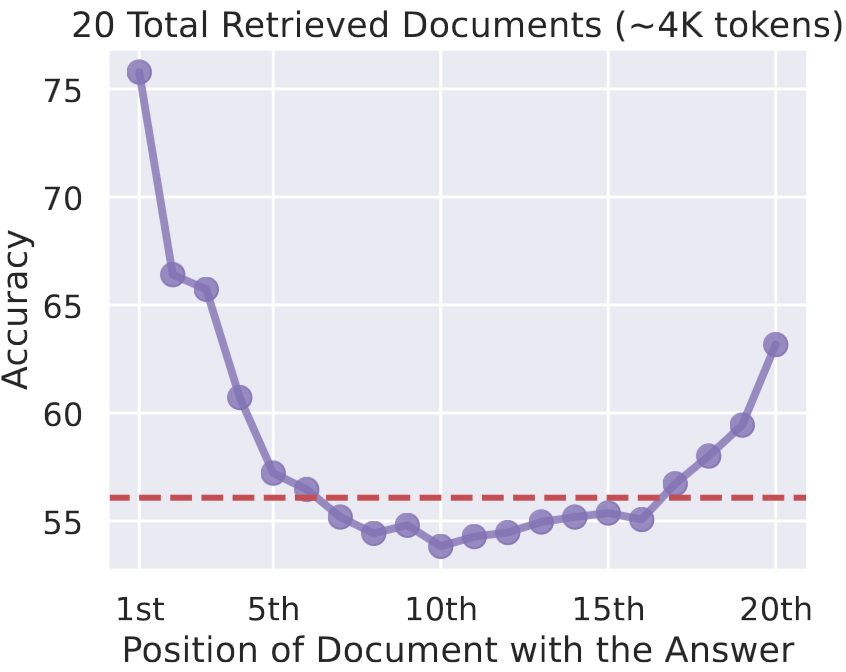
\includegraphics[width=0.5\textwidth]{./figuras/Precision_LLM_gran_contexto.png}
    \source{\cite{liuLostMiddleHow2023}}
    \label{fig:Precision_LLM_gran_contexto}
\end{figure}


Esto se debe a varios factores: En primer lugar, la ventana de contexto definitivamente limita la memoria del LLM (el número de \textit{tokens} que recibe como input para la siguiente respuesta) de forma que los primeros prompts, precisamente en los que se le daban las directrices generales para un obra, quedan fuera de su alcance. Su comportamiento en ese momento es impredecible, y tiende a enfocarse en las últimas tareas como objetivo principal. Y debido a que el usuario desconoce cuál es el valor de esta ventana de contexto, puede arrastrar el proyecto en la conversación hacia un punto sin salida. En segundo lugar, independientemente de la ventana de contexto, y especialmente en las ventanas grandes, se ha visto que los LLM no procesan por igual toda la información. Pueden existir lagunas importantes en el centro de la ventana, tal como demuestran recientes estudios \citep{liuLostMiddleHow2023}, lo cual puede llevar al modelo a alucinar. La Figura \ref{fig:Precision_LLM_gran_contexto} muestra una gráfica con este fenómeno. Por tanto, en una conversación larga dentro de la creación de un proyecto de envergadura el LLM puede sufrir de pérdida absoluta de la parte inicial de la conversación (limitación de la ventana de contexto) y, por otra parte, de pérdida parcial de la parte central de la conversación (limitación de la precisión en el centro de la ventana de contexto). Si a esto le sumamos que el usuario desconoce el valor de la ventana de contexto en el caso de chatGPT, el resultado es que el usuario puede arrastrar el proyecto hacia un punto sin salida, en el que el LLM no recuerda las directrices iniciales y puede alucinar en el centro de la ventana de contexto. Véase la Figura \ref{fig:chat_ventana_lost_in_the_middle}, que ilustra gráficamente el problema combinado de conocimiento del contexto por parte de los LLM en conversaciones suficientemente largas.


\begin{figure}[h!]
    \caption[Ventana de contexto y pérdida de precisión en su interior]{Ventana de contexto y pérdida de precisión en su interior. En un proyecto de medianas y grandes dimensiones, chatGPT puede perder la memoria de las directrices iniciales (limitación de la ventana de contexto) y perder precisión o alucinar en el centro de la ventana de contexto (limitación de la precisión en el centro de la ventana de contexto). Las partes sombreadas indican una pérdida total (fuera de la ventana de contexto) o parcial (hacia la mitad de la ventana de contexto) de la atención por parte del LLM.}
    \centering
    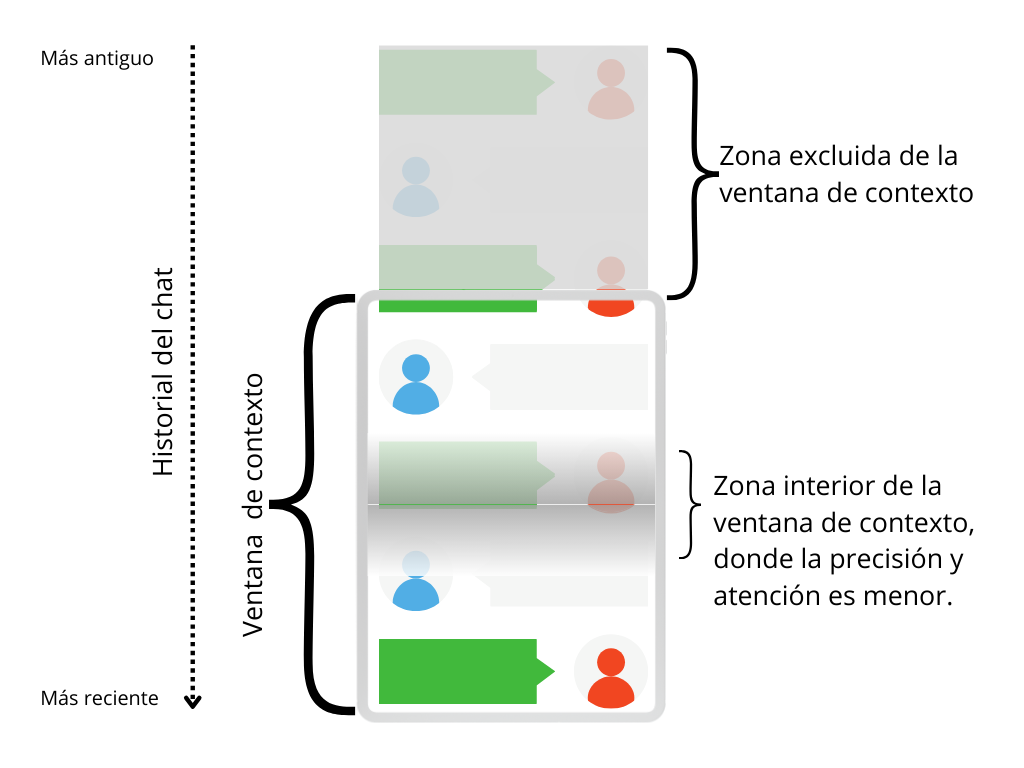
\includegraphics[width=0.7\textwidth]{./figuras/chat_ventana_lost_in_the_middle.png}
    \source{Elaboración propia.}
    \label{fig:chat_ventana_lost_in_the_middle}
\end{figure}


\subsection{Creación de bloques sencillos de código}

Nos referimos con <<bloque>> a una pieza de código funcional, pero que no constituye un proyecto completo, como, por ejemplo, una función, un patrón, etc. Al no constituir un código completo, no se requiere del manejo de una gran información en las respuestas del LLM, por lo que se puede esperar una mayor precisión en las mismas, al tiempo que se evitan los problemas asociados con la ventana de contexto. Del mismo modo, el usuario, a priori, puede controlar mejor la conversación iterando de una forma más controlada y cómoda. 

Esta forma de trabajo, sin embargo, requiere de una buena planificación por parte del usuario, en la medida en la que es este quien dará unidad a los diferentes elementos del trabajo sonoro y musical. En este sentido, es difícil pensar en un buen rendimiento de este flujo de trabajo sin conocimientos sólidos de las herramientas de programación utilizadas. Si bien existen técnicas de uso de LLM que implican la interacción de varios modelos o conversaciones paralelas, al modo de <<agentes>>, en este trabajo no se ha explorado esta posibilidad debido a su complejidad y a la falta de técnicas y plataformas maduras que permitan su uso \footnote{Con relación a técnicas de <<agentes>> aplicadas a la generación de código, véase \cite{huangAgentCoderMultiAgentbasedCode2023}. Un repositorio con extensa y actualizada bibliografía sobre el tema puede encontrarse en \cite{AGIEdgerunnersLLMAgentsPapers2024}.}

En general, en nuestros experimentos se ha encontrado que GPT-4 se ha desenvuelto con notable corrección en sus respuestas en el sentido sintáctico, mostrando una alta capacidad de autocorrección cuando se le ha devuelto un código de error, requiriendo poca o nula intervención humana en la corrección de errores. No obstante, como ocurría en el caso de la creación de esbozos generales de una obra, se han encontrado casos de bloqueo en la conversación, en los que el LLM no ha sido capaz de avanzar en la tarea sin la intervención humana. 

El lenguaje utilizado para comunicarse con GPT-4 siempre ha sido, deliberadamente, el lenguaje natural orientado a la creación sonora y musical, con el fin de encontrar así los límites de esta herramienta. Incluso en el caso de conversaciones en las que se devuelve código correcto y funcional, se han encontrado diversos problemas a nivel artístico, que hay que tener muy en cuenta a la hora de utilizar esta herramienta con fines musicales y que pasamos a detallar.

% \begin{itemize}
%     \item Alucinaciones recurrentes.
%     \item Abuso de valores <<por defecto>>, que restan interés artístico al código.
%     \item Errores indetectables y potencialmente peligrosos.
%     \item Introducción de errores de sintaxis en código previamente correcto.
%     \item Ocasionales errores de sintaxis que escapan a la autocorrección.
%     \item Gran distancia entre el sonido producido y el sonido esperado.
% \end{itemize}

\subsubsection{Alucinaciones recurrentes}
Las <<alucinaciones>> en los LLM son una de las características más conocidas de estos modelos, al tiempo que una de las más difíciles de detectar sin una supervisión humana, y, por ende, uno de los mayores handicups a la hora de delegar tareas de cualquier índole a sistemas de IA. Se entiende por <<alucinación>> a un dato erróneo que el modelo genera con total apariencia de veracidad y corrección. En el mejor de los casos estas alucinaciones se producen en el uso de clases o métodos inexistentes en el lenguaje de programación en uso. Normalmente estos defectos son fáciles de detectar por el compilador o por el intérprete del lenguaje, que suele dar cuenta de dicho problema inmediatamente. Por ejemplo, en el caso de SuperCollider, un código como el de la Figura \ref{fig:alucinacion_chatgpt} es correcto desde el punto de vista sintáctico, pero no lo es desde el punto de vista de la semántica del lenguaje, ya que utiliza la clase \texttt{KarplusStrong}, que no existe en SuperCollider. En este caso, el intérprete de SuperCollider dio buena cuenta de este error. 

\begin{figure}[H]
    \caption[Alucinación de ChatGPT utilizando una clase que no existe]{Alucinación de ChatGPT utilizando una clase que no existe ante el prompt <<Crea una textura sonora en supercollider inspirándote en el modelado físico de sonido.>> ChatGPT utiliza como base el UGen \texttt{KarplusStrong}, el cual no existe en SuperCollider.}
    \centering
    \setstretch{1}
    \begin{lstlisting}[style=SuperCollider-IDE, basicstyle=\footnotesize\ttfamily, numbers=none]
// Crear una función para el sonido modelado físicamente
(
SynthDef(\ksTexture, {
    arg freq=440, amp=0.5, gate=1, pan=0;
    var env, sig;
    env = EnvGen.kr(Env.adsr(0.01, 0.1, 0.6, 0.4), gate, doneAction: 2);
    // Crear el sonido utilizando KarplusStrong
    sig = KarplusStrong.ar(freq, 0.5, 0.1, 1, env);
    sig = Pan2.ar(sig * amp, pan);
    Out.ar(0, sig);
}).add;
)
    \end{lstlisting}
    \source{Elaboración propia.}
    \label{fig:alucinacion_chatgpt}
\end{figure}


Encontramos aún errores semánticos más sutiles y difíciles de detectar, ya que requieren de un conocimiento profundo del lenguaje de programación en uso y el intérprete no encuentra, pudiendo pasar desapercibidos, lo cual puede ser considerado un problema de seguridad. Un ejemplo claro es cuando la amplitud de la salida de audio satura el sistema. Los lenguajes de programación sonora no cuentan a priori con limitaciones de volumen o frecuencia, por lo que un error de este tipo puede provocar daños en el equipo de sonido o en el oído del usuario (véase Figura \ref{fig:amplitud_saturada_chatgpt}). Similar a este error es, en SuperCollider, la acumulación de instancias de un \texttt{Synth} en el servidor de audio, lo cual puede provocar un bloqueo del sistema. En la Figura \ref{fig:error_dificil_detectar_supercollider} se puede ver un ejemplo de este tipo de error. En este caso, el usuario ha tenido que intervenir para corregir el código generado por el modelo. Junto a la <<alucinación>>, se trata de uno de los problemas que pueden pasar desapercibidos cuando no existe un entendimiento profundo del lenguaje por parte del usuario.

\begin{figure}[H]
    \caption[Código saturado en amplitud, generado por ChatGPT]{Código saturado en amplitud, generado por ChatGPT. El código generado por ChatGPT es correcto desde el punto de vista sintáctico, pero la amplitud de la señal de audio satura el sistema. Este tipo de errores no son detectados hasta que se ejecuta el código, y son potencialmente peligrosos para el equipo de sonido o el oído del usuario.}
    \centering
    \setstretch{1}
    \begin{lstlisting}[style=SuperCollider-IDE, basicstyle=\footnotesize\ttfamily, numbers=none]
(
    {
        var x, y, z, a, b, c, d, e, f, g, h, mix;
        
        x = SinOsc.ar((Decay.ar(Impulse.ar([4,4.005]), 1e3*MouseX.kr(0, 1).abs)*50), MouseY.kr(0, 1)).distort;
        y = BPF.ar(Saw.ar([40,40.001]), LFNoise0.kr(128)+1*4e3+146, LFNoise1.kr(1)+1*5e-2+0.01).tanh;
        z = DelayC.ar(LPF.ar(LFNoise0.ar(8)**2 + x.tanh.round(0.05), 6e3), 1, LFNoise0.ar(8!2).range(1e-4, 0.02));
        a = BHiPass.ar(LFNoise1.ar(8)**3, y.midicps, y/2e3, 67-y);
        b = PitchShift.ar(Saw.ar(Demand.kr(Impulse.kr(4), 0, Drand(([-12, -7, 0, 7, 12]+33).midicps, inf)), Decay.kr(Impulse.kr(4), 3)), 7, 2);
        c = Impulse.ar(8)*LFNoise1.ar(2);
        d = Limiter.ar(GVerb.ar(BPF.ar(c, [400, 800], 1/9, 50).tanh, 100, 10), 0.9);
        mix = Mix.new([x, y, z, a, b, c, d]);
        Out.ar(0, Splay.ar(mix));
    }.play;
)
            
    \end{lstlisting}
    \source{Elaboración propia.}
    \label{fig:amplitud_saturada_chatgpt}
\end{figure}


\begin{figure}[H]
    \caption[Error difícil de detectar en SuperCollider]{Error difícil de detectar en SuperCollider: El \texttt{Synth} \texttt{\textbackslash dual\_osc} no cuenta con mecanismo de autoliberación, por lo que se acumulan ilimitadas instancias en el servidor de audio llamadas desde el bucle \texttt{loop} hasta saturar el sistema. Este código fue creado por ChatGPT y posteriormente autocorregido tras pasarle la información del error.}
    \centering
    \setstretch{1}
    \begin{lstlisting}[style=SuperCollider-IDE, basicstyle=\footnotesize\ttfamily, numbers=none]
(
    SynthDef(\dual_osc, {
        arg out=0, freq1=440, freq2=660, amp1=0.5, amp2=0.5;
        var sig;
        sig = SinOsc.ar([freq1, freq2], 0, [amp1, amp2]);
        Out.ar(out, sig);
    }).add;
    )
    // --- código intermedio omitido por brevedad ---
    {
        loop {
            var freq1, freq2, amp1, amp2;
            freq1 = freqPattern1.next * 400 + 100;
            freq2 = freqPattern2.next * 400 + 100;
            amp1 = ampPattern1.next;
            amp2 = ampPattern2.next;
            Synth(\dual_osc, [\freq1, freq1, \freq2, freq2, \amp1, amp1, \amp2, amp2]);
            0.1.wait;
        }
    }.fork;
)
    \end{lstlisting}
    \source{Elaboración propia.}
    \label{fig:error_dificil_detectar_supercollider}
\end{figure}

\subsubsection{Abuso de valores <<por defecto>>}
Otro defecto observado con relación a los parámetros de los métodos y clases del código es la propensión a utilizar valores por defecto. Esto, aunque no compromete la seguridad, resta interés al código generado desde el punto de vista artístico. Los valores por defecto son aquellos que un elemento del código utiliza cuando el usuario no provee de un valor explícito. Por ejemplo, en el caso de SuperCollider, el método \texttt{SinOsc.ar} cuenta con un parámetro \texttt{mul} que, si no se provee de un valor explícito, toma el valor por defecto de 1; o \texttt{freq}, con el valor por defecto de \SI{440}{\hertz}. Por ejemplo, en la Figura \ref{fig:ChatGPT_valores_por_defecto} se puede ver cómo el modelo utiliza valores por defecto en el código generado, lo cual no es deseable desde el punto de vista artístico. Junto a la <<alucinación>>, se trata de uno de los problemas que pueden pasar desapercibidos sin un entendimiento profundo del lenguaje por parte del usuario, si bien puede mitigarse a través del uso de técnicas de \textit{prompting}, como se verá más adelante.

\begin{figure}[H]
    \caption[]{Código generado por ChatGPT con utilización de valor de frecuencia de 440 Hz. Este valor <<por defecto>> no es una excepción, sino que sistemáticamente se encuentran enn los parámetros de los métodos y clases del código generados por ChatGPT. Esto, sin duda, resta interés al código generado desde el punto de vista artístico.}
    \centering
    \setstretch{1}
    \begin{lstlisting}[style=SuperCollider-IDE, basicstyle=\footnotesize\ttfamily, numbers=none]
(
    SynthDef(\fmSound, {
        arg freq=440, amp=0.5, modIndex=5, attackTime=0.01, releaseTime=1;
        var carrier, modulator, env;
    
        // Envolvente
        env = EnvGen.kr(Env.perc(attackTime, releaseTime), doneAction:2);
    
        // Modulador
        modulator = SinOsc.ar(freq, 0, modIndex);
    
        // Portadora
        carrier = SinOsc.ar(freq + modulator) * amp;
    
        // Salida
        Out.ar(0, carrier * env);
    }).add;
    
    // Toca el sonido
    Synth(\fmSound, [
        \freq, 440, // Frecuencia en Hz
        \amp, 0.5, // Amplitud
        \modIndex, 5, // Índice de modulación
        \attackTime, 0.01, // Tiempo de ataque en segundos
        \releaseTime, 1 // Tiempo de liberación en segundos
    ]);
) 
    \end{lstlisting}
    \source{Elaboración propia.}
    \label{fig:ChatGPT_valores_por_defecto}
\end{figure}



\subsubsection{Introducción de errores de sintaxis en código previamente correcto}
Aunque infrecuente, no menos desconcertante es la introducción impredecible de errores de cualquier tipo en código previamente correcto. Si los errores son de sintaxis, el compilador o el intérprete del lenguaje darán cuenta de ellos, pero si se trata de errores de semántica, como en el caso de la alucinación, pueden pasar desapercibidos. La introducción de nuevos errores en código previo es un problema que aparece según la conversación, o el tamaño del código, es comparable al tamaño de la ventana de contexto. De nuevo, el nivel de conocimientos de usuario es fundamental para detectar este tipo de errores.


\subsubsection{Ocasionales errores de sintaxis que escapan a la autocorrección}
Una característica interesante de los LLM es la de autocorregirse. Esto es, si el usuario le devuelve un el mensaje de error dado por el sistema, el modelo es capaz de corregirlo en la siguiente respuesta. Sin embargo, factores que escapan al control, como la introducción de alucinaciones, problemas con la ventana de contexto o la simple carencia de información de entrenamiento en el problema actual del código, pueden hacer que el modelo no sea capaz de autocorregirse, pudiendo llevar a un bloqueo en la conversación, especialmente si esta se extiende demasiado en relación a su ventana de contexto, donde, como vimos, se producen lagunas de información. En relación a esto, se han encontrado errores de sintaxis muy simples, como ausencia de paréntesis, que el modelo no ha sido capaz de diagnosticar.


\subsubsection{Gran distancia entre el sonido producido y el sonido esperado}
El poder de los LLM es del procesar el lenguaje natural y traducir descripciones en código funcional. Si el código requerido es el de una función, digamos, en \textit{Python}, que ha de <<devolver el sumatorio de las entradas>>, el nivel de comprensión requerido al LLM en dicha transcripción es trivial, en tanto en cuanto la propia descripción es prácticamente un pseudocódigo de dicha función. El desnivel semántico no es comparable cuando lo que pedimos al LLM es <<crear un sonido rugoso que evolucione temporalmente de la granulación a un sonido armónico con leves y agradables fluctuaciones de sus componentes parciales>>. En este caso, el LLM ha de comprender la descripción, traducirla a código y, además, generar un sonido que se adecue a la descripción.  En este caso, el desnivel semántico es mucho mayor ya que la descripción responde a criterios estéticos y psicoacústicos, por lo que el resultado puede ser muy distinto al esperado. En la Figura \ref{fig:ChatGPT_desnivel_semantico} se puede ver un ejemplo de este fenómeno. Este problema puede ser mitigado en parte con el uso de técnicas de prompting y una continua iteración en la conversación, pero en muchos casos el resultado final el resultado aceptado por el usuario puede estar lejos el esperado, lo cual constituye un problema a la hora de usar esta herramienta para la creación musical. La Figura \ref{fig:ChatGPT_desnivel_semantico} muestra un ejemplo de este fenómeno. Aparentemente, el código representa un conjunto de sonidos naturales de un bosque, pero el resultado es ruido blanco. 

\begin{figure}[H]
    \caption[Desnivel semántico de ChatGPT en un código en SuperCollider]{Desnivel semántico de ChatGPT en un código en SuperCollider. El código aparentemente representa un conjunto de sonidos naturales de un bosque, pero el resultado es ruido blanco de alto nivel de amplitud, totalmente alejado del significado semántico de la descripción.}
    \centering
    \setstretch{1}
    \begin{lstlisting}[style=SuperCollider-IDE, basicstyle=\footnotesize\ttfamily, numbers=none]
(
    // Definir los componentes del paisaje sonoro
    var arroyo, pajaros, viento, hojas;
    
    // Arroyo: Ruido blanco filtrado
    arroyo = { BPZ2.ar(WhiteNoise.ar(0.3), 1000) };
    
    // Pájaros: Tonos agudos y aleatorios
    pajaros = { SinOsc.ar([4000, 4500].choose, 0, 0.1) * EnvGen.ar(Env.perc(0.01, 0.1), Impulse.kr([5, 7].choose)) };
    
    // Viento: Ruido rosa
    viento = { PinkNoise.ar(0.2) };
    
    // Hojas y Ramas: Ruido blanco con envolventes
    hojas = { WhiteNoise.ar(0.1) * EnvGen.ar(Env.perc(0.005, 0.1), Impulse.kr(10)) };
    
    // Mezclar y reproducir todos los componentes
    { arroyo!2 + pajaros!2 + viento!2 + hojas!2 }.play;
)
            
    \end{lstlisting}
    \source{Elaboración propia.}
    \label{fig:ChatGPT_desnivel_semantico}
\end{figure}

A nivel artístico, la utilización de esta herramienta con conocimiento de la misma, así como del campo en cuestión, en este caso, la creación sonora y musical. La creación iterada de snippets de código sonoro puede producir fragmentos de código eventualmente de interés, en muchos casos como serendipia, si bien, al menos en el momento de la realización de este trabajo, esta valoración artística entra ya en la percepción estética y subjetiva del creador humano.


\subsection{Influjo del uso de técnicas de \textit{prompting} en ChatGPT}

En la sección \ref{sec:llm_tecnicas_prompting} se han descrito algunas de las técnicas más relevantes en cuanto al prompting de un \gls{llm}, especialmente las que han presentado buenos resultados en aritmética y generación de código de programación, como \gls{cot}. De igual modo, en \ref{sec:llm_asistentes_creacion_codigo_programacion} se presentaban técnicas avanzadas como \gls{scot} en la generación de código.

A continuación se analiza, de forma cualitativa y descriptiva, el impacto que han tenido diferentes técnicas de \textit{prompting} en las respuestas obtenidas del modelo.

\subsubsection{\textit{Zero-shot} vs \textit{Few-shot}}

Aunque ChatGPT está entrenado para establecer conversaciones tipo chat, es susceptible de recibir contextos junto a la petición del usuario con un conjunto de ejemplos de código, para que el modelo pueda aprender de ellos para elaborar su respuesta. En este sentido, se ha encontrado que la presentación de ejemplos de código al modelo tiene un efecto positivo en cuanto estilo y formato del código, incluso en el uso de elementos de programación similares a dichos ejemplos, siendo menos proclive a errores sintácticos. Sin embargo, no se ha encontrado que el uso de ejemplos de código mejore la calidad del código generado en el sentido artístico. 

La Figura \ref{fig:chatgpt_zero_shot_vs_few_shot} muestra el resultado de una misma petición a ChatGPT con \textit{Zero-shot} y \textit{One-shot}. El resultado es claramente positivo en el segundo caso. Como veremos, este resultado es clave para el éxito en la utilización de técnicas más avanzadas, como \gls{rag}.


\begin{figure}%[H]
    \caption[]{Comparación de resultados de ChatGPT con (a) \textit{Zero-shot} y (b) \textit{Few-shot}.}
    \centering
    \begin{subfigure}{.48\textwidth}
      \centering
      \begin{mdframed}
        \setstretch{1}
        Usuario: Crea una textura sonora de interés artístico usando \texttt{FMGrain} en SuperCollider.
      \end{mdframed}
    %   \caption{Csound}
    \end{subfigure}\hfill
    \begin{subfigure}{.48\textwidth}
      \centering
      \begin{mdframed}
        \setstretch{1}
        Usuario: Crea una textura sonora de interés artístico usando \texttt{FMGrain} en SuperCollider. Te paso un ejemplo de uso:
        \begin{lstlisting}[style=SuperCollider-IDE, basicstyle=\footnotesize\ttfamily, numbers=none]
SynthDef(\fm_grain_test, {arg gate = 1, amp = 1;
    Out.ar(0,
        FMGrain.ar(Impulse.ar(20), 0.2, 440, 200,
            LFNoise1.kr(1).range(1, 10),
            EnvGen.kr(
                Env([0, 1, 0], [1, 1], \sin, 1),
                gate,
                levelScale: amp,
                doneAction: 2)
        )
    )
}).add;
s.sendMsg(\s_new, \fm_grain_test, a=s.nextNodeID, 0, 1, \amp, 0.1);
        \end{lstlisting}
      \end{mdframed}
    %   \caption{SuperCollider}
    \end{subfigure}

    \vspace{0.2cm}

    \begin{subfigure}{.48\textwidth}
        \centering
        \setstretch{1}
        \begin{lstlisting}[style=SuperCollider-IDE, basicstyle=\footnotesize\ttfamily, numbers=none]
{
    var dur, dens, fund, form, indx, pan;
    dur = MouseX.kr(0.01, 0.2, 1, 0.01); 
    dens = MouseY.kr(20, 50, 1, 0.1);
    fund = 200;                     
    form = 800;
    indx = 2;
    pan = LFNoise2.kr(0.5).range(-1, 1); 

    FMGrain.ar(
        numChannels: 2,
        trigger: Impulse.kr(dens),
        dur: dur,
        carfreq: fund,
        modfreq: form,
        index: indx,
        pan: pan
    )
}.play;    
        \end{lstlisting}
        \caption{
        \begin{tabular}{@{}p{0.7\textwidth}p{0.2\textwidth}@{}}
            \textit{Zero-shot} en una petición de creación sonora en SuperCollider. & 
            \qrcode[height=1.5cm]{https://drive.google.com/file/d/13AMMKehJHzlI8CQUqCqoWMHZ9AI2YgcS/view?usp=drive_link}
        \end{tabular}
        }
      \end{subfigure}\hfill
    \begin{subfigure}{.48\textwidth}
      \centering
        \setstretch{1}
        \begin{lstlisting}[style=SuperCollider-IDE, basicstyle=\footnotesize\ttfamily, numbers=none]
SynthDef(\fm_grain_artistic, { arg gate = 1, amp = 1;
    var sound, freq, dur, pan, rate, index;

    // Parámetros modificables para la textura
    freq = LFNoise1.kr(0.5).range(200, 1000);
    dur = LFNoise2.kr(0.1).range(0.1, 0.5); 
    pan = LFNoise2.kr(0.2).range(-1, 1); 
    rate = LFNoise1.kr(0.3).range(5, 50); 
    index = LFNoise1.kr(0.4).range(100, 800); 

    // Creación de la textura sonora
    sound = FMGrain.ar(
        Impulse.ar(rate), dur, freqindex, 5,pan               
    );

    // Aplicación del envolvente y salida
    Out.ar(0,
        Pan2.ar(
            sound * EnvGen.kr(
                Env([0, 1, 0], [0.1, 0.1], \sin, 1),
                gate,
                levelScale: amp,
                doneAction: 2
            ),
            pan
        )
    );
}).add;
s.sendMsg(\s_new, \fm_grain_artistic, a=s.nextNodeID, 0, 1, \amp, 0.1);              
        \end{lstlisting}
        \caption{
        \begin{tabular}{@{}p{0.7\textwidth}p{0.2\textwidth}@{}}
            La misma petición con un ejemplo \textit{Few-shot}. El resultado sonoro es más interesante desde el punto de vista artístico. & 
            \qrcode[height=1.5cm]{https://drive.google.com/file/d/1C7FDkH706e1OMlcOWrG4qsCoC7Au8GaU/view?usp=drive_link}
        \end{tabular}
        }
    \end{subfigure}

    \source{Elaboración propia.}
    \label{fig:chatgpt_zero_shot_vs_few_shot}
\end{figure}

\subsubsection{\textit{Chain of Thoughts} (CoT) y \textit{Structured Chain of Thoughts} (SCoT)}

Esta técnica requiere de un nivel mayor de abstracción en el razonamiento del \gls{llm}, al exigirle una planificación previa a la implementación del código. Esto implica la elaboración de la respuesta en dos pasos, una para la planificación y razonamiento, y otra, para la implementación en sí. Dichos pasos pueden ser dados en una sola respuesta o en dos. En el caso de ChatGPT, o el de cualquier chat de \gls{ia}, a cuyos parámetros de respuesta no podemos acceder, conviene hacerlo en dos respuestas consecutivas para asegurarnos de no alcanzar un límite de \textit{tokens} en la única respuesta. 

A diferencia de \textit{Few-shot}, esta técnica no mejora la respuesta del \gls{llm} de forma drástica, pero sí que se aprecian cambios positivos en cuanto a la complejidad de elementos que el código puede llegar a utilizar. Así, una petición compleja del usuario tiene más probabilidades de éxito si el \gls{llm} tiene la posibilidad de <<razonar>> previamente los pasos a dar que si lo implementa directamente. A cambio, puede introducir más errores en el código, que el usuario ha de corregir por sí mismo o llevar al \gls{llm} en una conversación iterada. Esta técnica es más apropiada que \textit{Few-shot} en el caso de buscar un código para una pieza en evolución temporal, donde se implican estructuras tipo rutinas, patrones y cambios de parámetros o sintetizadores a lo largo del tiempo, aunque, será útil en cualquier aplicación en la que se busque complejidad. En los experimentos realizados se han desechado muchas conversaciones completas por llegar a momentos de bloqueo, en los que la complejidad del código era tal que su depuración era más costosa que la elaboración del mismo a partir de partes más pequeñas.

No se ha mostrado como relevante el uso de una técnica tipo \gls{scot}, en la que el primer paso ha de realizarse en pseudocódigo en lugar de en lenguaje natural. La hipótesis que lanzamos para este resultado es que, a diferencia de las tareas de programación a las que esta técnica originalmente se dirige, el diseño de sintetizadores no requiere de tanta complejidad como una función en Python o C++ que se descompone en flujos como bucles y condicionales. En este sentido, el propio script en SuperCollider se representa a sí mismo y no tiene sentido planificar en un pseudocódigo.

\subsubsection{\textit{Self-Debugging}}

Una aproximación para intentar minimizar los errores sintácticos del código generado podría ser el ya expuesto \textit{Self-Debugging}, en el que el \gls{llm} ha de dar un paso posterior a la implementación en código para revisar los posibles errores del código. En ninguno de los casos que se ha utilizado se han corregido errores algunos. La única forma de que el \gls{llm} corrija sus errores es que el usuario le devuelva el mensaje de error del compilador o del intérprete del lenguaje, en cuyo caso el \gls{llm} comprenderá el problema y tratará de resolverlo en la siguiente respuesta. 

De hecho, este es un flujo habitual en el que se desenvuelve las conversaciones de creación sonora con ChatGPT. La inmensa mayoría de los bloques de código generados con éxito en este trabajo, han sido realizados de forma iterativa, limpiando el código a partir de los mensajes de error devueltos por el intérprete de SuperCollider. En este punto, el papel del usuario compositor y su nivel de conocimientos es fundamental para el éxito de la tarea. La Figura \ref{fig:iteracion_depuracion} muestra este proceso en bucle en el que el usuario devuelve al \gls{llm} los mensajes de error iterativamente.

\begin{figure}[H]
    \caption[Iteración de depuración de código con ChatGPT]{Iteración de depuración de código con ChatGPT. El usuario devuelve al LLM los mensajes de error iterativamente.}
    \centering
    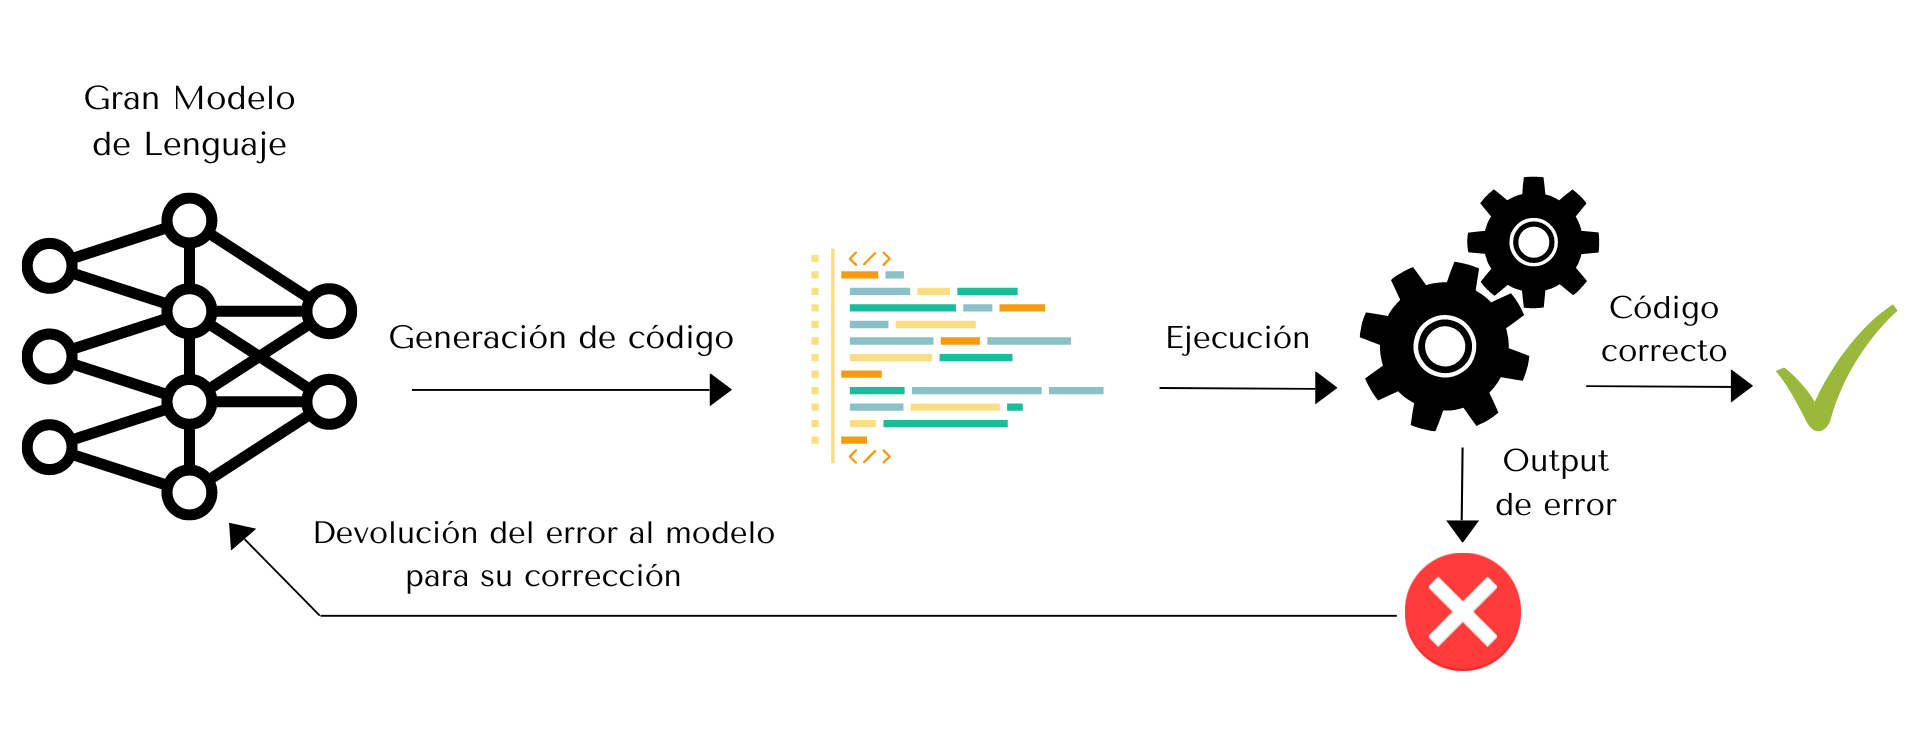
\includegraphics[width=0.9\textwidth]{./figuras/iteracion_depuracion_codigo.png}
    \source{Elaboración propia.}
    \label{fig:iteracion_depuracion}
\end{figure}

\subsubsection{Uso de \textit{Retrieval-Augmented Generation} (RAG)}


\section{Mayor control de parámetros con el Playground de OpenAI}

\section{Ampliando el \textit{Knowledge}: RAG con \textit{GPTs} y \textit{Assistants}}

\section{Programando con la API de OpenAI}
Aquí se explica con detalle los scripts que se han programado, dificultades, limitaciones y puntos de interés.






% ----Ejemplos sonoros conseguidos a través de ChatGPT.